

\documentclass[runningheads]{llncs}

\usepackage{graphicx}
\usepackage{times}
%\usepackage{rotate}
%\usepackage{lscape}

\begin{document}

\frontmatter          % for the preliminaries
\pagestyle{headings}  % switches on printing of running heads
\mainmatter              % start of the contributions
\title{Projet de G\'enie Logiciel\\
Rapport de Planification\\
Ann\'ee Acad\'emique 2014-2015}

\titlerunning{Rapport de planification -- \textbf{2014-2015}}

\author{Groupe num\'ero: \textbf{7}\\
Membres du groupe: \textbf{DELGRANGE FLORENT, LECOQ ALEXIS, LEMPEREUR MARTIN}}
%
\authorrunning{Groupe \textbf{7} - \textbf{BAC 2}} 

\institute{\textbf{BAC 2 INFO}\\
Facult\'e des Sciences, Universit\'e de Mons\\
\email{martin.lempereur@hotmail.be}
%VOUS POUVEZ UTILISER UN AUTRE ADRESSE MAIL QUE CELUI DE L'UMONS SI VOUS LE PREFERIEZ
}

\maketitle              % typeset the title of the contribution

\begin{center} \today \end{center}

Ce rapport de planification est rendu dans le cadre du cours ``Projet de G\'enie Logiciel" (dispens\'e par le Prof. \emph{Tom Mens} en ann\'ee acad\'emique 2014-2015). Le but de ce rapport est d'expliquer quels sont les objectifs
du projet, quelles sont les diff\'erentes t\^aches a r\'ealiser et planifier c'est diff\'erentes t\^aches.


\newpage
%%%%%%%%%%%%%%%%%%%%%%%%%%%%%%%%%%%%%%%%%%%%%%%%
%%%%%%%%%%%%%%%%%%%%%%%%%%%%%%%%%%%%%%%%%%%%%%%%
\section{Introduction}\label{sec:intro}

\subsection{Objectifs}
%%Quels sont le contexte et les objectifs du projet de g\'enie logiciel?
Le travail s'inscrit dans le cadre du projet de G\'enie logiciel.
\newline Le travail consiste \`a concevoir un jeu de r\^ole dont l'unvivers est celui de l'Unviversit\'e.
\newline Nous conceverons donc une application java et ce en d\'ecomposant la r\'ealisation  en plusieurs \'etapes cl\'es.


%%%%%%%%%%%%%%%%%%%%%%%%%%%%%%%%%%%%%%%%%%%%%%%%
\subsection{Exigences fonctionnelles}

\emph{Quelle est la fonctionnalit\'e demand\'e du logiciel \`a d\'evelopper?}

BLA BLA BLA

%%%%%%%%%%%%%%%%%%%%%%%%%%%%%%%%%%%%%%%%%%%%%%%%
\subsection{Exigences non-fonctionnelles}

%%\emph{Quelles sont les exigences sur la qualit\'e (p.e. portabilit\'e, fiabilit\'e, s\^uret\'e, extensibilit\'e, modularit\'e, performance  ou autre)?}

L'application doit \^etre executable sur les syst\`emes exploitation Linux, Mac et Windows.
\newline Le jeu de r\^ole pourra supporter l'ajout de qu\^etes, de caract\`eristiques et m\^eme de classes.

%%%%%%%%%%%%%%%%%%%%%%%%%%%%%%%%%%%%%%%%%%%%%%%%
\subsection{Contraintes de temps}

\emph{Quels sont les contraintes sur l'emploi du temps? (Dates d'\'ech\'eance, vacances, examens, autres cours et projets, ...)? Si vous le d\'esirez vous pouvez utiliser une table pour clarifier l'emploi du temps. Vous pouvez \'egalement ajouter une figure.}

BLA BLA BLA

%%%%%%%%%%%%%%%%%%%%%%%%%%%%%%%%%%%%%%%%%%%%%%%%
\subsection{Contraintes de budget}

\emph{Quels sont les contraintes sur le budget \`a d\'epenser? Pou chaque achat ou d\'pense, justifiez la n\'ecessit\'e de l'achat et du cout.}

BLA BLA BLA

\newpage
%%%%%%%%%%%%%%%%%%%%%%%%%%%%%%%%%%%%%%%%%%%%%%%%
%%%%%%%%%%%%%%%%%%%%%%%%%%%%%%%%%%%%%%%%%%%%%%%%
\section{Ressources}\label{sec:organisation}

\subsection{Les ressources humaines (personnel)}

\emph{Qui va travailler sur le projet? Quels sont les membres de l'\'equipe? Y a-t-il d'autres parties prenantes (stakeholders) qui ont un int\'er\^et dans le projet? (N'oubliez pas le professeur et les assistants.) Quel est le r\^ole et la responsabilit\'e de chacun? Quel est l'effort fourni par chaque personne (par exemple, plein temps, mi-temps \`a 50\%, etc.)}

\emph{Si vous le d\'esirez vous pouvez utiliser une table ici, comme la table~\ref{tab:RH}.}

\begin{table}[!htbp]
\begin{center}
\begin{tabular}{p{1.5cm}|p{1.5cm}|p{1.5cm}|p{2cm}|p{2cm}|p{1.5cm}}
nom & r\^ole & dur\'ee & responsabilit\'e \\
\hline
Florent Delgrange & r\'ealiser le projet & environ 8 mois & conception de l'\'interace graphique, impl\'ementation du framework & \\
Martin Lempereur  & r\'ealiser le projet & environ 8 mois & impl\'ementation du framework & \\
Alexis Lecoq  & r\'ealiser le projet & environ 8 mois & impl\'ementation du framework & \\
\end{tabular}
\end{center}
   \caption{Ressources humaines.}
   \label{tab:RH}
\end{table}

%%%%%%%%%%%%%%%%%%%%%%%%%%%%%%%%%%%%%%%%%%%%%%%%
\subsection{Les ressources logicielles}

\emph{Quels logiciels seront utilis\'es et pourquoi? Pr\'excisez les caract\'�ristiques de chaque logiciel: son nom, son co\^ut, sa version, son utilit\'e, son type de licence, \ldots.}

\emph{Y a-t-il des logiciels suppl\'ementaires \`a procurer? Estimer le d\'elai et les co\^ut de ces logiciels.}

\emph{Y a-t-il des contraints sur les logiciels ou mat\'eriels \`a utiliser (par exemple, \`a cause de compatibilit\'e et interop\'erabilit\'e avec d'autres syst\`emes existants)? Les choix effectu\'es ici devront \^etre conformes aux exigences de la section~\ref{sec:intro}.}

\emph{Si vous le d\'esirez vous pouvez utiliser une table ici.}

BLA BLA BLA

%%%%%%%%%%%%%%%%%%%%%%%%%%%%%%%%%%%%%%%%%%%%%%%%
\subsection{Les ressources mat\'erielles}

\emph{Quelles machines seront utilis\'ees? Pr\'excisez les caract\'�ristiques de chaque mat\'eriel: le nom, le co\^ut, le plateforme d'exploitation, le m\'empire, le processeur, le disque dur ou SSD, \ldots}

\emph{Y a-t-il des mat\'eriaux suppl\'ementaires \`a procurer? Estimer le d\'elai et les prix de ces mat\'eriaux.}

\emph{Les machines de d\'eveloppement seront-elles diff\'erentes des machines de d\'eploiement? Si c�est le cas,  d\'ecrivez les caract\'eristiques de chacun.}

\emph{Les choix effectu\'es ici devront \^etre conforme aux contraintes et exigences de la section~\ref{sec:intro}.}

BLA BLA BLA

%%%%%%%%%%%%%%%%%%%%%%%%%%%%%%%%%%%%%%%%%%%%%%%%
%%%%%%%%%%%%%%%%%%%%%%%%%%%%%%%%%%%%%%%%%%%%%%%%
\newpage
\section{Analyse des risques}

\subsection{Identification des risques}\label{sec:riskident}

\emph{Quels sont les risques potentiels du projet? Classifiez les risques par cat\'egorie (par exemple les risques li\'es au personnel, au produit, au projet; d'autres classifications sont permises).  Distinguez les risques g\'en\'eriques (au moins 4), applicables \`a tout projet (informatique), des risques sp\'ecifiques (au moins 4) pour votre propre projet. Donnez une description textuelle de chaque risque.}

\emph{Prioritisez les risques selon leur importance, en fonction de leur probabilit\'e et s\'ev\'erit\'e. Vous devez justifier la probabilit\'e et s\'ev\'erit\'e de chaque risque.
Si vous le souhaitez, vous pouvez utiliser une table pour r\'esumer les risques retenus, comme par exemple la Table~\ref{tab:risques}.}


\begin{table}[!htbp]
\begin{center}
\begin{tabular}{|p{3cm}||c|c|}
\hline
\textbf{Risque} & Probabilit\'e & S\'ev\'erit\'e\\
\hline\hline
risque 1 & basse &  non significative \\
\hline
risque 2 & \Large{haute} &  tol\'erable \\
\hline
risque 3 & \large{mod\'er\'ee} & \large{s\'erieuse} \\
\hline
risque 4 & basse & \Large{catastrophique} \\
\hline
\end{tabular}
\end{center}
   \caption{Analyse des risques.}
   \label{tab:risques}
\end{table}

%\`A titre d'information, voici quelques exemples de risques souvent rencontr\'es dans un projet informatique:
%\begin{itemize}
%\item difficult\'es techniques impr\'evues (probl\`eme de versions, probl\`eme de compatibilit\'e, mat\'eriel ou logiciel d\'efectueux, perte de donn\'ees, ...)
%\item difficult\'e de compr\'ehension (documentation non disponible en fran\c{c}ais, documentation absent, sujet ou domaine complex et difficile \`a ma\^itriser, ...)
%\item probl\`eme de ressources (mat\'erial non disponible, indisponibilit\'e du directeur ou autres personnes impliqu\'ees dans le travail, manque de communication)
%\item probl\`eme d'horaire (manque de temps, horaire de cours inflexible, maladie, ...)
%\item probl\`eme du produit final (incompl\`ete, peu performant, instable, d\'efectueux, manque de documentation, difficile \`a utiliser ou maintenir, probl\`eme de fiabilit\'e ou s\'ecurit\'e, ...)
%\end{itemize}
%
%Cette liste \textbf{n'est pas exhaustive} et peut varier selon le contexte du travail. Ce qui est important se sont les risques qui sont vraiment sp\'ecifiques \`a votre projet.

%%%%%%%%%%%%%%%%%%%%%%%%%%%%%%%%%%%%%%%%%%%%%%%%
\subsection{Gestion des risques}\label{sec:riskmanagement}

Pour chaque risque que vous avez retenu dans la section \ref{sec:riskident} (en fonction de son importance), expliquez comment vous comptez 
\begin{enumerate}
\item \'eviter que le risque se produira
\item v\'erifier si le risque s'est produit
\item r\'esoudre ou r\'eduire l'ampleur du risque quand il s'est produit
\end{enumerate}

%%%%%%%%%%%%%%%%%%%%%%%%%%%%%%%%%%%%%%%%%%%%%%%%
%%%%%%%%%%%%%%%%%%%%%%%%%%%%%%%%%%%%%%%%%%%%%%%%
\newpage
\section{R\'epartition du travail}

\subsection{Work Breakdown Structure}

\emph{Mettez la r\'epartition des t\^aches et sous-t\^aches, ou l'horaire du projet ici. Indiquez \'egalement qui fait quelle t\^ache.
Pour ce faire, vous pouvez inclure une figure ici (extrait d'un outil de planification), ou vous pouvez mettre les informations dans un tableau de t\^aches, comme par exemple Table~\ref{tab:WBS}.}

\begin{table}[htbp]
\begin{center}
\begin{tabular}{|r|p{4cm}||p{2cm}|p{2cm}|c|c|c|}
\hline
\textbf{ID} & T\^ache & Dates & Responsable & \% travail & Autre remarques\\
\hline\hline
T1 & \'etablir le cahier de charges &  & ... l'\'etudiant ... & 100\% &\\
\hline
\hline
T2 & description t\^ache 2 & & &  & \\
\hline
T3 & description t\^ache 3 & & & &\\
\hline
\end{tabular}
\end{center}
   \caption{Tableau des t\^aches.}
   \label{tab:WBS}
\end{table}

%%%%%%%%%%%%%%%%%%%%%%%%%%%%%%%%%%%%%%%%%%%%%%%%
\subsection{Etapes cl\'es }

\emph{Quels sont les \'etapes cl\'es (milestones)? Quelles sont les livrables (si pr\'esent) pour chaque \'etape cl\'e? Donnez une description du contenu de chaque livrable.
Vous pouvez utiliser un tableau d'\'etapes cl\'es pour repr\'esenter une partie de l'information requise, comme par exemple Table~\ref{tab:TEC}.}

\begin{table}[htbp]
\begin{center}
\begin{tabular}{|c||c|c|c|}
\hline
Date & \'etape cl\'e & Livrables\\
\hline\hline
31 octobre & r\'eunion d'inspection de la planification de projet & rapport de planification  \\
\hline
 & &  \\
\hline
 & &  \\
\hline
\end{tabular}
\end{center}
   \caption{Tableau d'\'etapes cl\'es.}
   \label{tab:TEC}
\end{table}

%%%%%%%%%%%%%%%%%%%%%%%%%%%%%%%%%%%%%%%%%%%%%%%%
%%%%%%%%%%%%%%%%%%%%%%%%%%%%%%%%%%%%%%%%%%%%%%%%
\newpage
\section{Ordonnancement}

\subsection{Diagramme GANTT}

\emph{Vous devriez inclure et discuter ici un ou plusieurs diagrammes de GANTT, comme ceux montr\'es dans les Figures~\ref{fig:GANTT} et~\ref{fig:GANTT2}. \`A vous de choisir comment g\'en\'erer le(s) diagramme(s). Pr\'ecisez le ou les outils utilis\'es pour la cr\'eation de chaque diagramme.}

\begin{figure}[!htb]
\begin{center}
%%  \includegraphics[width=\textwidth]{GANTT.jpg}
  \caption{Exemple d'un diagramme GANTT.}\label{fig:GANTT}
\end{center}
\end{figure}

\begin{figure}[!htb]
\begin{center}
%%  \includegraphics[width=\textwidth]{GANTT2.jpg}
  \caption{Un autre exemple d'un diagramme GANTT.}\label{fig:GANTT2}
\end{center}
\end{figure}

\emph{N'oubliez pas d'indiquer, sur le diagramme, les \'etapes cl\'es et les d\'ependances entre les t\^aches. Si l'outil que vous avez utilis\'e ne permet pas de faire cela, vous pouvez mettre cette information dans une table s\'epar\'ee, comme par exemple Table~\ref{tab:GANTT}.}

\begin{table}[htbp]
\begin{center}
\begin{tabular}{|p{2cm}||c|c||c|}
\hline
\textbf{T\^ache} & Pr\'edecesseurs \\
\hline\hline
id tache 1 &   \\
\hline
id tache 2 &  \\
\hline
id tache 3 & \\
\hline
\end{tabular}
\end{center}
   \caption{D\'ependances entre les t\^aches.}
   \label{tab:GANTT}
\end{table}

%%%%%%%%%%%%%%%%%%%%%%%%%%%%%%%%%%%%%%%%%%%%%%%%
\subsection{Diagramme PERT}

\emph{Vous devriez inclure et discuter ici un ou plusieurs diagrammes  PERT, comme ceux montr\'es dans les Figure~\ref{fig:PERT} et Figure~\ref{fig:PERT2}. \`A vous de choisir comment g\'en\'erer ce diagramme. Pr\'ecisez le ou les outils utilis\'es pour la cr\'eation de chaque diagramme.}

\begin{figure}[!htb]
\begin{center}
%%  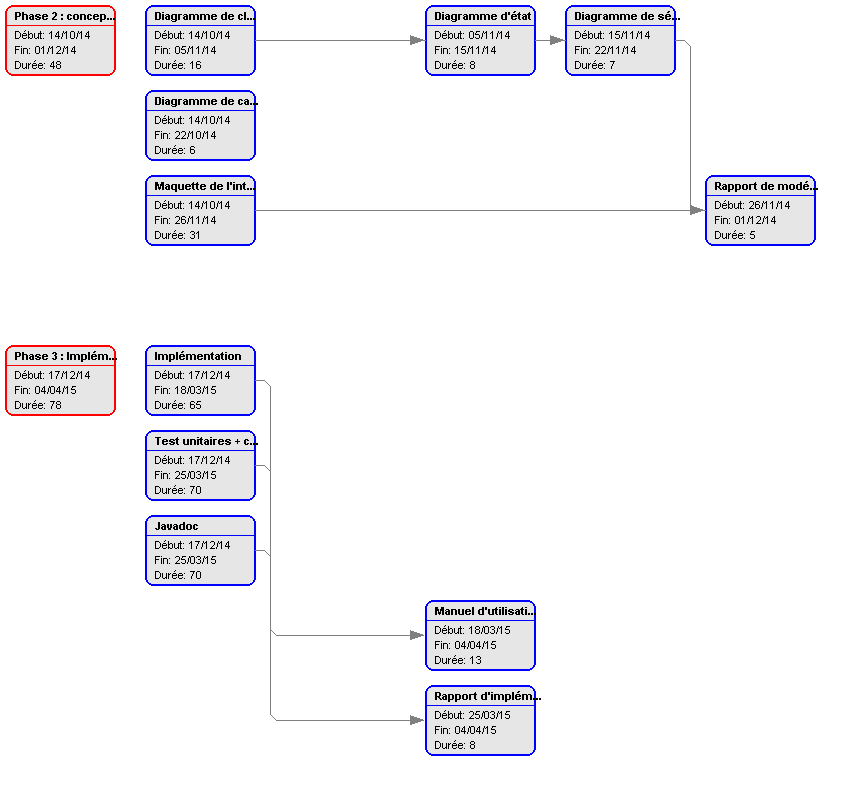
\includegraphics[width=\textwidth]{PERT.jpg}
  \caption{Exemple d'un diagramme PERT.}\label{fig:PERT}
\end{center}
\end{figure}

\begin{figure}[!htb]
\begin{center}
%%  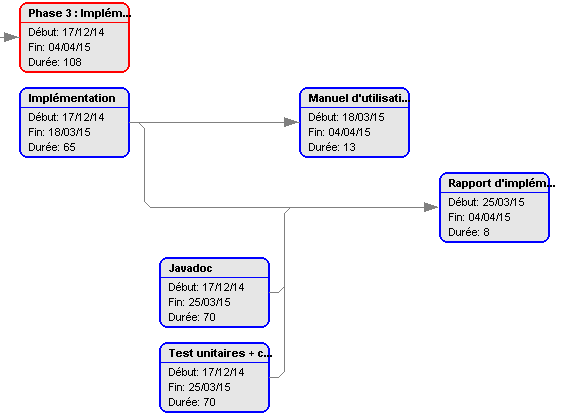
\includegraphics[width=\textwidth]{PERT2.jpg}
  \caption{Un autre exemple d'un diagramme PERT.}\label{fig:PERT2}
\end{center}
\end{figure}

Si l'outil que vous avez utilis\'e pour g\'en\'erer le diagramme PERT le permet, vous devriez indiquer dans le diagramme, pour chaque t\^ache, la dur\'ee, l'effort (en personne/mois), le temps "Earliest Start (ES)", le temps "Latest Start (LS)", le temps l\^ache (\emph{Slack Time (ST)}), et le \emph{Free Float (FF)}. Le diagramme doit \'egalement montrer o\`u se trouve le(s) chemin(s) critique(s).

Si l'outil que vous avez utilis\'e ne le permet pas vous devriez mettre ces informations dans une table s\'epar\'ee, comme par exemple la Table~\ref{tab:PERT}.

\begin{table}[htbp]
\begin{center}
\begin{tabular}{|p{2cm}||c|c|c|c|c|c|}
\hline
\textbf{T\^ache} & Dur\'ee & Effort & Earliest Start & Latest Start & Slack Time & Free Float\\
\hline\hline
nom tache 1 & D1 & EFF1 & ES1 & LS1 & ST1 & FF1 \\
\hline
nom tache 2 & D2 & EFF2 & ES2 & LS2 & ST2 & FF2 \\
\hline
nom tache 3 & D3 & EFF3 & ES3 & LS3 & ST3 & FF3 \\
\hline
\end{tabular}
\end{center}
   \caption{Informations temporelles importantes sur les t\^aches.}
   \label{tab:PERT}
\end{table}

%%%%%%%%%%%%%%%%%%%%%%%%%%%%%%%%%%%%%%%%%%%%%%%%
\subsection{Analyse de l'ordonnancement}

\emph{Analysez les diagrammes en calculant le chemin critique, les temps l\^aches (marge totale) et la marge libre (free float), tout en v\'erifiant que vous avez fait un bon choix. (Si non, vous devriez modifier votre ordonnancement afin de l'optimiser...)
Justifiez votre d\'ecision.}

%%%%%%%%%%%%%%%%%%%%%%%%%%%%%%%%%%%%%%%%%%%%%%%%
\subsection{Surveillance}

\emph{Expliquez comment vous comptez surveiller les retards \'eventuels du projet quand il est en cours de route. Quelle proc\'edure allez vous suivre pour d\'etecter et \'eviter ces retards? Qu'allez vous faire quand un retard se manifeste?}

\emph{Expliquez \'�galement comment vous comptez surveiller les risques.}

\bibliographystyle{splncs}
\bibliography{biblio}

\end{document}
